\documentclass[14pt,a4paper]{article}
\usepackage[14pt]{extsizes}
\usepackage[left=1.5cm, right=1.5cm, top=1.5cm, bottom=1.5cm]{geometry}
\usepackage[utf8]{inputenc}
\usepackage[T2A]{fontenc}
\usepackage[english, russian]{babel}
\usepackage{amsmath,amsfonts,amssymb,amsthm,mathtools} 
\usepackage{amsfonts}
\usepackage{amssymb}
\usepackage{titleps}
\usepackage{hyperref}
\usepackage{float}
\usepackage{graphicx}
\usepackage{multirow}
\usepackage{hhline}
\usepackage{wrapfig}
\usepackage{tikz}
\usepackage{pgfplots}
\usepackage{xcolor}
\usepackage{subfig}
\usepackage{upgreek}

\newcommand{\w}[1]{\text{#1}}
\newcommand{\und}[1]{\underline{#1}}
\newcommand{\img}[3]{
	\begin{figure}[H]
	\begin{center}
	\includegraphics[scale=#2]{#1}
	\end{center}
	\begin{center}
 	\textit{#3}
	\end{center}
	\end{figure}
}
\newcommand{\aw}[1]{
	\begin{center}
	\textit{#1}
	\end{center}
	\n
}
\newcommand{\be}[1]{
	\begin{center}
	\boxed{#1}
	\end{center}
}
\newcommand{\beb}[1]{
	\begin{equation}
	\boxed{#1}
	\end{equation}
}
\newcommand{\eb}[1]{
	\begin{equation}
	#1
	\end{equation}
}
\newcommand{\n}{\hfill \break}
\newcommand{\x}{\cdot}

\begin{document}
\begin{titlepage}
	\begin{center}
		{\large МОСКОВСКИЙ ФИЗИКО-ТЕХНИЧЕСКИЙ ИНСТИТУТ (НАЦИОНАЛЬНЫЙ ИССЛЕДОВАТЕЛЬСКИЙ УНИВЕРСИТЕТ)}
	\end{center}
	
	\vspace{4.5cm}
	{\huge
		\begin{center}
			{\bf Отчёт о выполнении лабораторной работы 3.2.3}\\
			Резонанс токов в параллельном контуре
		\end{center}
	}
	\vspace{2cm}
	\begin{flushright}
		{\LARGE Авторы:\\ Клименко Виталий Евгеньевич \\ Киркича Андрей Александрович \\
			\vspace{0.2cm}
			Б01-202}
	\end{flushright}
	\vspace{3.8cm}
	\begin{center}
		Долгопрудный\\
		\today
	\end{center}
\end{titlepage}
\n
	\textbf{Цель работы: }
	исследование резонанса токов в параллельном колебательном контуре с изменяемой ёмкостью, получение амплитудно-частотных и фазово-частотных характеристик, определение основных параметров контура.
	\n\n
	\textbf{В работе используются: }
	генератор сигналов, источник напряжения, нагрузкой которого является параллельный колебательный контур с переменной ёмкостью, двухканальный осциллограф, цифровые вольтметры.
	\subsection*{Теоретичские сведения и описание установки}
	В данной работе изучаются резонансные явления в параллельном колебательном контуре (резонанс токов). Блок-схема экспериментальной установки показана на рис. 1. Синусоидальный сигнал от генератора поступает на вход управляемого напряжением источника тока, собранного на операционном усилителе с полевым транзистором, питание которого осуществляется встроенным блоком–выпрямителем от сети ~220 В (цепи питания на схеме не показаны). Внутреннее
(выходное) сопротивление источника тока, бесконечно большое в идеальном случае, в нашей схеме составляет несколько ГОм. Это обеспечивает постоянство амплитуды тока $I$ на меняющейся нагрузке - параллельном контуре, изображённом на рис. 1 в виде эквивалентной схемы.
	\img{pic_1.png}{1.7}{Рис. 1: схема экспериментальной установки}
	\n
	Источник тока, колебательный контур и блок питания заключены в
отдельный корпус, отмеченный на рисунке штриховой линией. На корпусе имеются коаксиальные разъёмы «Вход», «$U_1$» и «$U_2$», а также переключатель магазина ёмкостей $C_n$, $n$ = 1 . . . 7. Величины ёмкостей $C_n$ и сопротивления $R_1$ указаны на установке. Напряжение $\varepsilon = \varepsilon_0 \cos(\omega t + \varphi_0)$
от генератора поступает на вход источника тока. Это же напряжение
через разъём «$U_1$» подаётся на канал 1 осциллографа и на вход вольтметра 1. Переменное напряжение на сопротивлении $R_1$ в используемой схеме равно напряжению $\varepsilon$ на выходе генератора и совпадает с ним по фазе. Следовательно, ток $I$ во внешней цепи параллельного контура определяется формулами:
	\eb{I = \frac{\varepsilon}{R_1} = I_0 \cos (\omega t + \varphi_0), \qquad I_0 = \frac{\varepsilon_0}{R_1}}
	\n
	Напряжение на контуре $U$, совпадающее с напряжением на конденсаторе $U_C$, поступает со знаком «–» через разделительный конденсатор и разъём «$U_2$» на канал 2 осциллографа, а также на вход вольтметра 2. Колебательный контур нашей установки собран из стандартных элементов, используемых в современных радиоэлектронных цепях. Получаем выражения для импедансов ёмкостной $Z_C$ и индуктивной $Z_L$ ветвей параллельного колебательного контура:
	\eb{Z_C = R_S - \frac{i}{\omega C}, \qquad Z_L = R + R_L + i \omega L}
	\aw{где $R_S$ и $R_L$ - активные части импендансов конденсатора и катушки индуктивности соответственно, а $R$ - величина постоянного активного сопротивления, добавленного в индуктивную ветвь колебательного контура для снижения его добротности с целью упрощения процедур получения и обработки резонансных кривых.}\n
	Конденсаторы магазина ёмкостей $C_n$ в интересующем нас диапазоне частот имеют относительно
малые потери.\n\n
Добротность $Q$ контуров в наших установках достаточно высока, cуммарное активное сопротивление контура в этом случае даётся формулой:
	\eb{R_{\Sigma} = R + R_L + R_S}
	и, следовательно:
	\eb{Q = \frac{\rho}{R_{\Sigma}} = \frac{\omega_0 L}{R_{\Sigma}} = \frac{1}{\omega_0 C R_{\Sigma}} >> 1}
	\n
	Сильное неравенство (4) в рабочем диапазоне частот выполняется для всех контуров, используемых в работе.\n\n
	Наибольший практический интерес для контуров с высокой добротностью ($Q >> 1$) представляет случай, когда отклонение $\Delta \omega = \omega - \omega_0$ частоты внешней ЭДС от собственной частоты контура удовлетворяет сильному неравенству:
	\eb{|\Delta \omega| << \omega_0}
	\n
	При этом в первом порядке малости по относительной расстройке частоты $\frac{\Delta \omega}{\omega_0}$ выполняется соотношение:
	\eb{\frac{\omega_0}{\omega_0} - \frac{\omega}{\omega} \approx \frac{2\Delta \omega}{\omega_0}}\n
	Величина $\delta \omega = 2 |\Delta \omega_{\gamma}| = 2\gamma = 2 / \tau$ представляет собой важную характеристику колебательного контура — ширину резонансной кривой U($\omega$), по которой с учётом соотношений $Q = \omega_0 / 2 \gamma = \tau \omega_0 / 2$, зная частоту $\omega_0$, можно найти добротность контура:
	\eb{Q = \frac{\omega_0}{\delta \omega}}\n
	Эти же параметры можно определить по фазово-частотной характеристике: тангенс угла наклона $\psi_U$ в точке $\omega = \omega_0$ определяет время затухания $\tau$, а расстояние по оси $\omega$ между точками, в которых фаза $\psi_U (\omega)$ меняется от $- \pi / 4$ до $\pi / 4$, равно $2 / \tau$ с относительной
погрешностью порядка $Q^{-2}$.
	\subsection*{Обработка результатов измерений}
	Для начала заполним таблицу, руководствуясь следующими формулами из теоретической справки:
\begin{equation}
    L = \frac{1}{C(2\pi f)^2}
\end{equation}
\begin{equation}
    \rho = \frac{1}{2 \pi f C}
\end{equation}
\begin{equation}
    |Z_{\text{рез}}|=\frac{U}{\mathcal{E}}R_1
\end{equation}
\begin{equation}
    Q = \frac{UR_1}{\mathcal{E}}2 \pi fC
\end{equation}
\begin{equation}
    R_{\Sigma} = \frac{\mathcal{E}}{UR_1} \frac{1}{(2 \pi fC)^2}
\end{equation}
\begin{equation}
    R_{S_{max}} = 10^{-3} \rho
\end{equation}
\begin{equation}
    R_L = R_{\Sigma} - R - R_{S_{max}}
\end{equation}
\begin{table}[H]
\caption{Основная таблица}
\centering
\resizebox{400pt}{!}{
\begin{tabular}{|r|r|r|r|r|r|r|r|r|r|r|r|}
\hline
\multicolumn{1}{|c|}{N} &
  \multicolumn{1}{c|}{$C$, нФ} &
  \multicolumn{1}{c|}{$f$, кГц} &
  \multicolumn{1}{c|}{$U$, В} &
  \multicolumn{1}{c|}{$\mathcal{E}$, В} &
  \multicolumn{1}{c|}{$L$, мГн} &
  \multicolumn{1}{c|}{$\rho$, Ом} &
  \multicolumn{1}{c|}{$|Z_{\text{рез}}|$, Ом} &
  \multicolumn{1}{c|}{$Q$} &
  \multicolumn{1}{c|}{$R_{\Sigma}$, Ом} &
  \multicolumn{1}{c|}{$R_{S_{max}}$, Ом} &
  \multicolumn{1}{c|}{$R_{L}$, Ом} \\ \hline
1                                             & 25,10                  & 32,00   & 1,50  & 0,30 & 986,52 & 198,25 & 5008,28 & 25,28 & 7,84 & 0,20 & 4,14 \\ \hline
2                                             & 33,20                  & 27,80 & 1,38 & 0,30  & 988,22 & 172,53 & 4606,09 & 26,71 & 6,46 & 0,17 & 2,78  \\ \hline
3                                             & 47,30                  & 23,00   & 0,99 & 0,30 & 1013,36 & 146,37  & 3303,28 & 22,58 & 6,48 & 0,15 & 2,83 \\ \hline
4                                             & 57,40                  & 21,00   & 0,85 & 0,30 & 1001,68 & 132,10 & 2836,15 & 21,48 & 6,15 & 0,13  & 2,51 \\ \hline
5                                             & 67,50                  & 19,40 & 0,70  & 0,30  & 998,10 & 121,60   & 2336,42 & 19,22 & 6,32 & 0,12  & 2,70 \\ \hline
6                                             & 82,70                  & 17,70 & 0,59 & 0,30  & 978,65 & 108,78 & 1969,27 & 18,11 & 6,00 & 0,11 & 2,39 \\ \hline
7                                             & 101,60                 & 16,10 & 0,48 & 0,30 & 962,80 & 97,35 & 1602,65 & 16,47 & 5,91 & 0,10 & 2,31 \\ \hline
\multicolumn{1}{|l|}{Ср. знач.}        & \multicolumn{1}{l|}{} &      &      &        & 989,91 &         &         &         &          &         & 2,81 \\ \hline
\multicolumn{1}{|l|}{Случ. погр.} & \multicolumn{1}{l|}{} &      &      &        & 16,49 &         &         &         &          &         & 0,62 \\ \hline
\end{tabular}
}
\end{table}
Рассчитаем средние значения $\langle L \rangle $ и $ \langle R_L \rangle $, а также их случайные погрешности $\Delta L$ и $\Delta R_L$ по формулам:
\begin{equation}
    \Delta L = \sqrt{\sum\limits_{i=1}^7(L_i-\langle L \rangle)^2}
\end{equation}
\begin{equation}
    \Delta R_L = \sqrt{\sum\limits_{i=1}^7(R_{L_i}-\langle R_L \rangle)^2}
\end{equation}
\n\n
Далее составим амплитудно-частотную характеристику для конденсаторов $C_2$ и $C_3$.
\begin{table}[H]
\caption{Данные для конденсатора $C_2$}
    \centering
    \begin{tabular}{|l|l|l|l|}
    \hline
        $U$, В & $f$, кГц & $U_{\text{отн}}$ & $f_{\text{отн}}$ \\ \hline
        0,83 & 28,43 & 0,60 & 1,02 \\ \hline
        0,90 & 28,32 & 0,65 & 1,02 \\ \hline
        0,95 & 28,25 & 0,69 & 1,02 \\ \hline
        1,00 & 28,18 & 0,72 & 1,01 \\ \hline
        1,06 & 28,09 & 0,77 & 1,01 \\ \hline
        1,08 & 28,05 & 0,78 & 1,01 \\ \hline
        1,10 & 28,03 & 0,80 & 1,01 \\ \hline
        1,15 & 27,90 & 0,83 & 1,00 \\ \hline
        1,14 & 27,80 & 0,83 & 1,00 \\ \hline
        1,09 & 27,68 & 0,79 & 1,00 \\ \hline
        1,02 & 27,50 & 0,74 & 0,99 \\ \hline
        0,97 & 27,45 & 0,70 & 0,99 \\ \hline
        0,93 & 27,40 & 0,67 & 0,99 \\ \hline
        0,90 & 27,36 & 0,65 & 0,98 \\ \hline
        0,85 & 27,29 & 0,62 & 0,98 \\ \hline
        0,82 & 27,26 & 0,59 & 0,98 \\ \hline
    \end{tabular}
\end{table}
\begin{table}[H]
    \centering
    \caption{Данные для конденсатора $C_3$}
    \begin{tabular}{|l|l|l|l|}
    \hline
        $U$, В & $f$, кГц & $U_{\text{отн}}$ & $f_{\text{отн}}$ \\ \hline
        0,60 & 22,57 & 0,61 & 0,98 \\ \hline
        0,67 & 22,68 & 0,68 & 0,99 \\ \hline
        0,74 & 22,77 & 0,75 & 0,99 \\ \hline
        0,77 & 22,81 & 0,78 & 0,99 \\ \hline
        0,83 & 22,88 & 0,84 & 0,99 \\ \hline
        0,85 & 22,91 & 0,86 & 1,00 \\ \hline
        0,88 & 22,95 & 0,89 & 1,00 \\ \hline
        0,90 & 22,97 & 0,91 & 1,00 \\ \hline
        0,97 & 23,32 & 0,98 & 1,01 \\ \hline
        0,86 & 23,48 & 0,87 & 1,02 \\ \hline
        0,82 & 23,54 & 0,83 & 1,02 \\ \hline
        0,81 & 23,56 & 0,82 & 1,02 \\ \hline
        0,77 & 23,60 & 0,78 & 1,03 \\ \hline
        0,66 & 23,76 & 0,67 & 1,03 \\ \hline
        0,65 & 23,79 & 0,66 & 1,03 \\ \hline
        0,61 & 23,84 & 0,62 & 1,04 \\ \hline
    \end{tabular}
\end{table}
По результатам измерений построим графики для обоих конденсаторов в осях $U(f)$ и $\frac{U}{U_0} (\frac{f}{f_0})$
\begin{figure}[H]
	\center{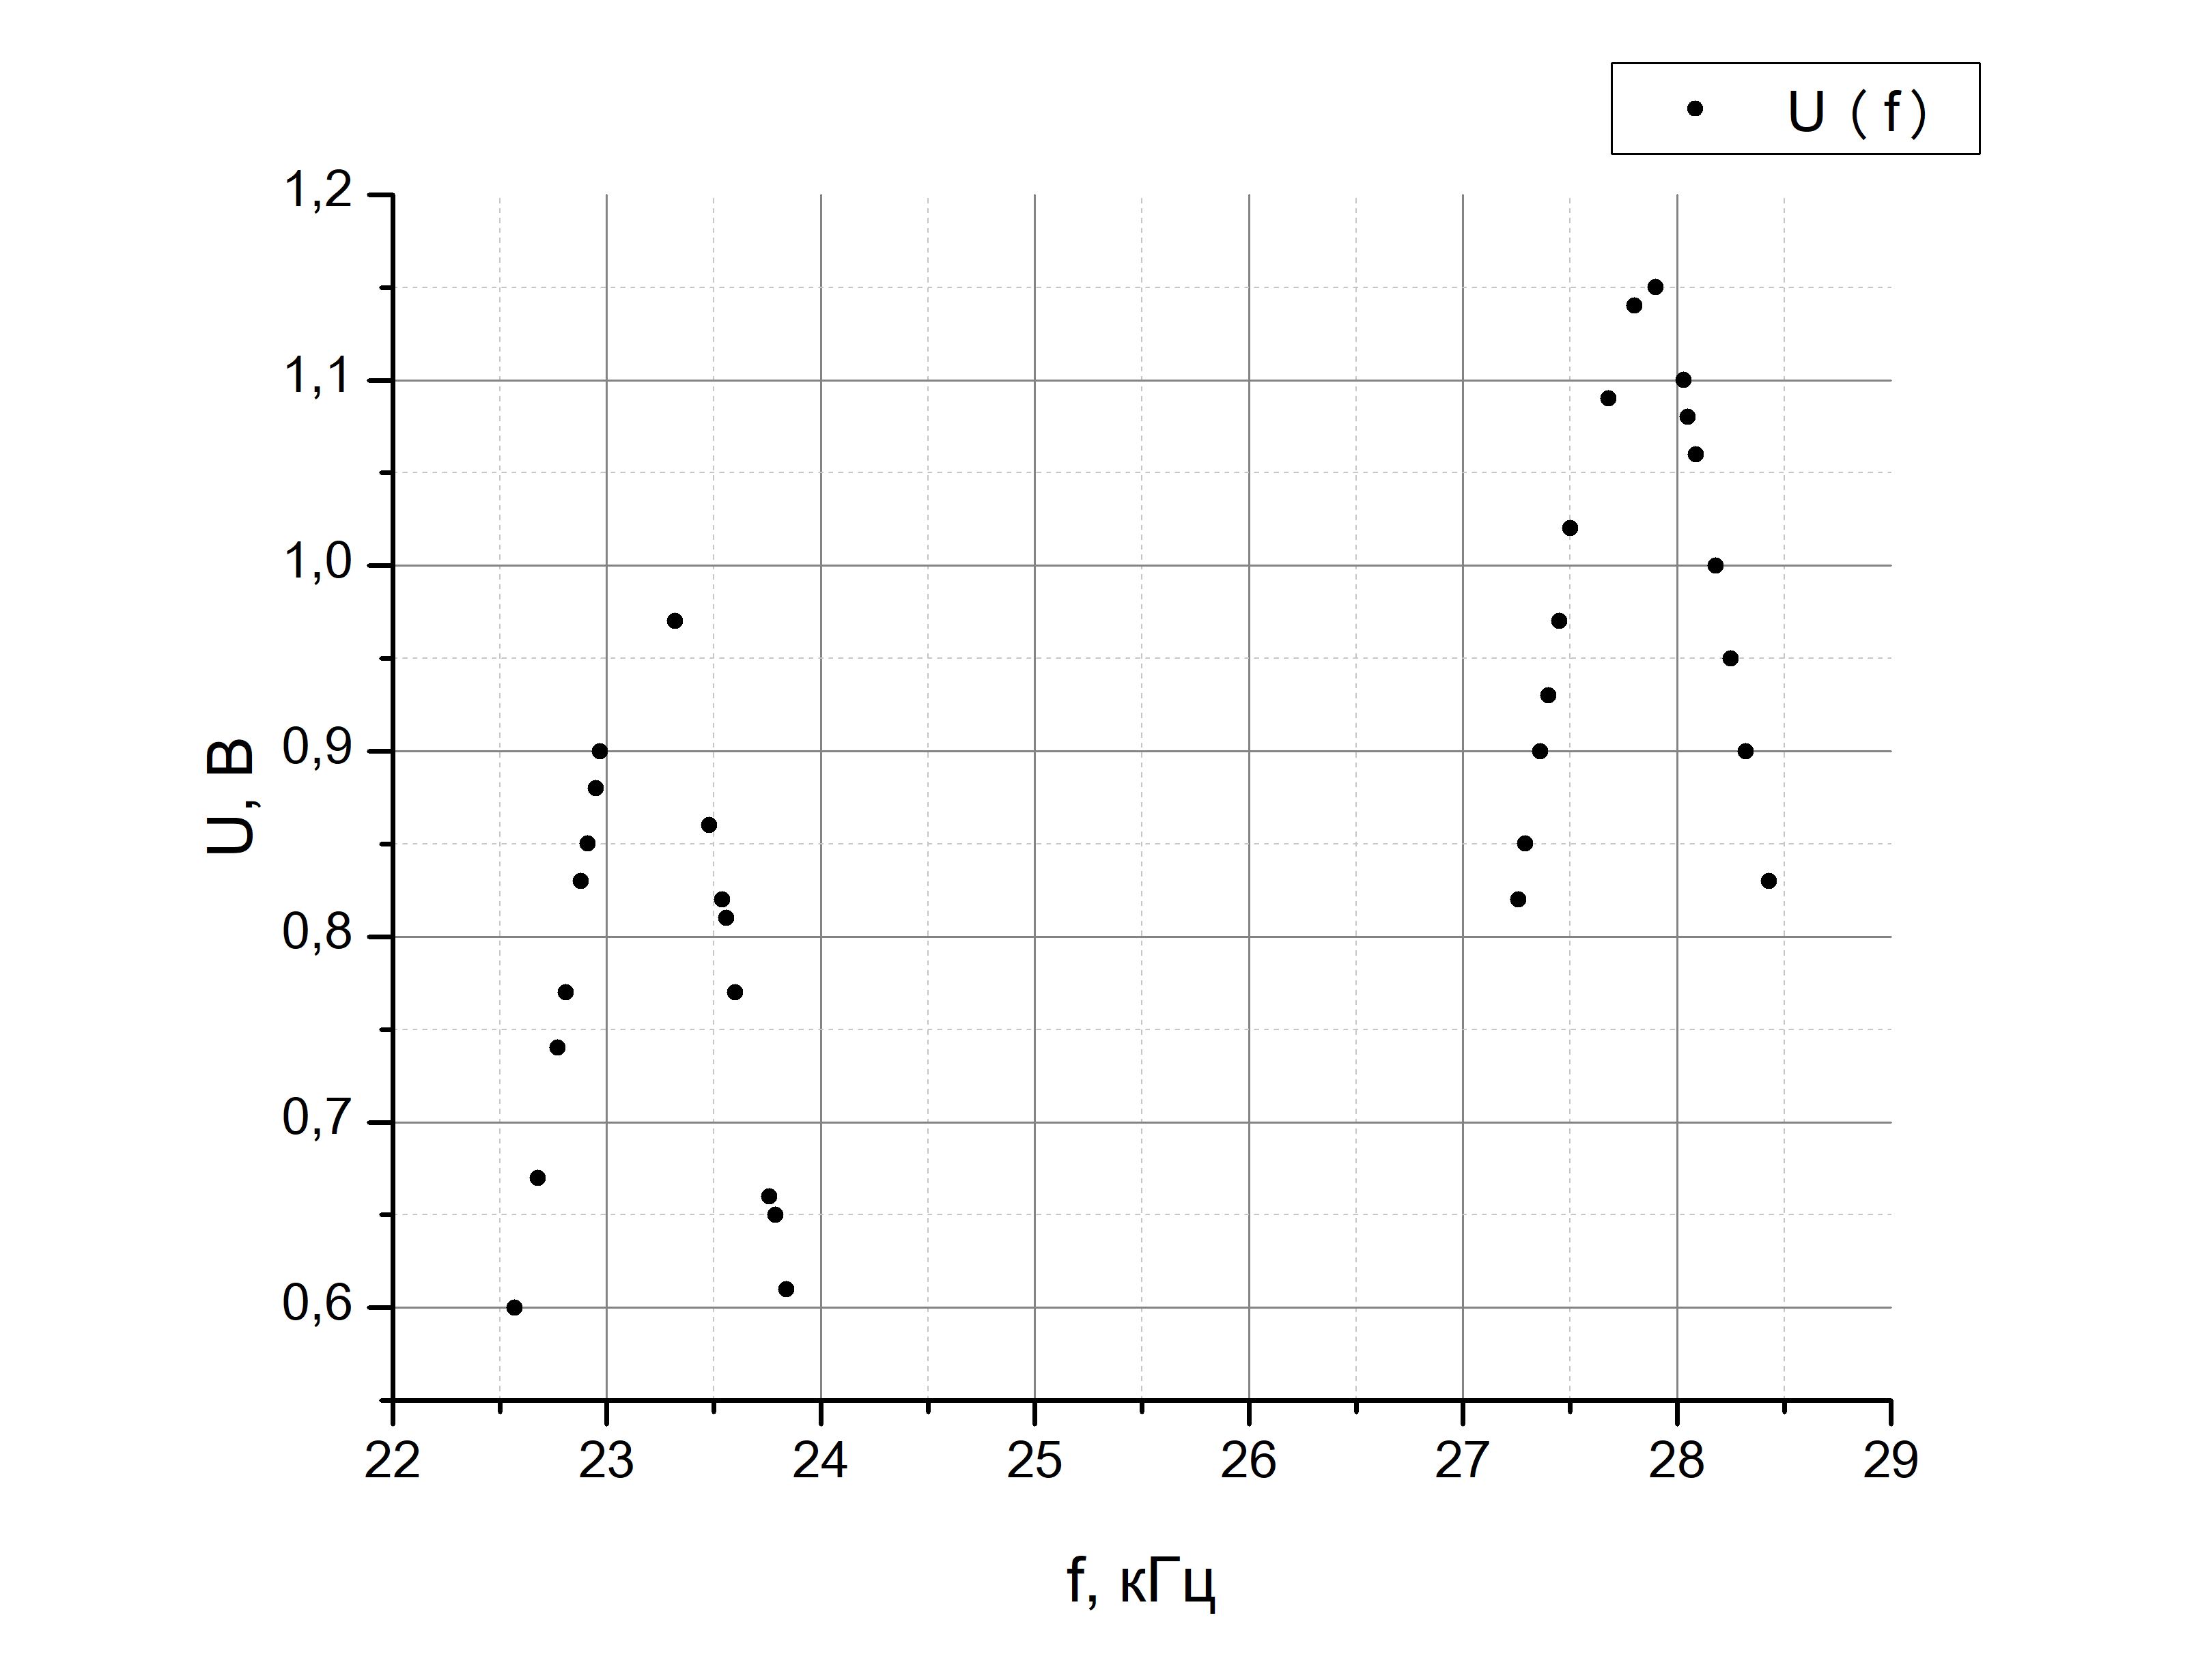
\includegraphics[scale=0.5]{АЧХ_1.png}}
	\caption{\centering График амплитудно-частотной характеристики в осях $U(f)$}
	\label{fig:image2}
\end{figure}
\begin{figure}[H]
	\center{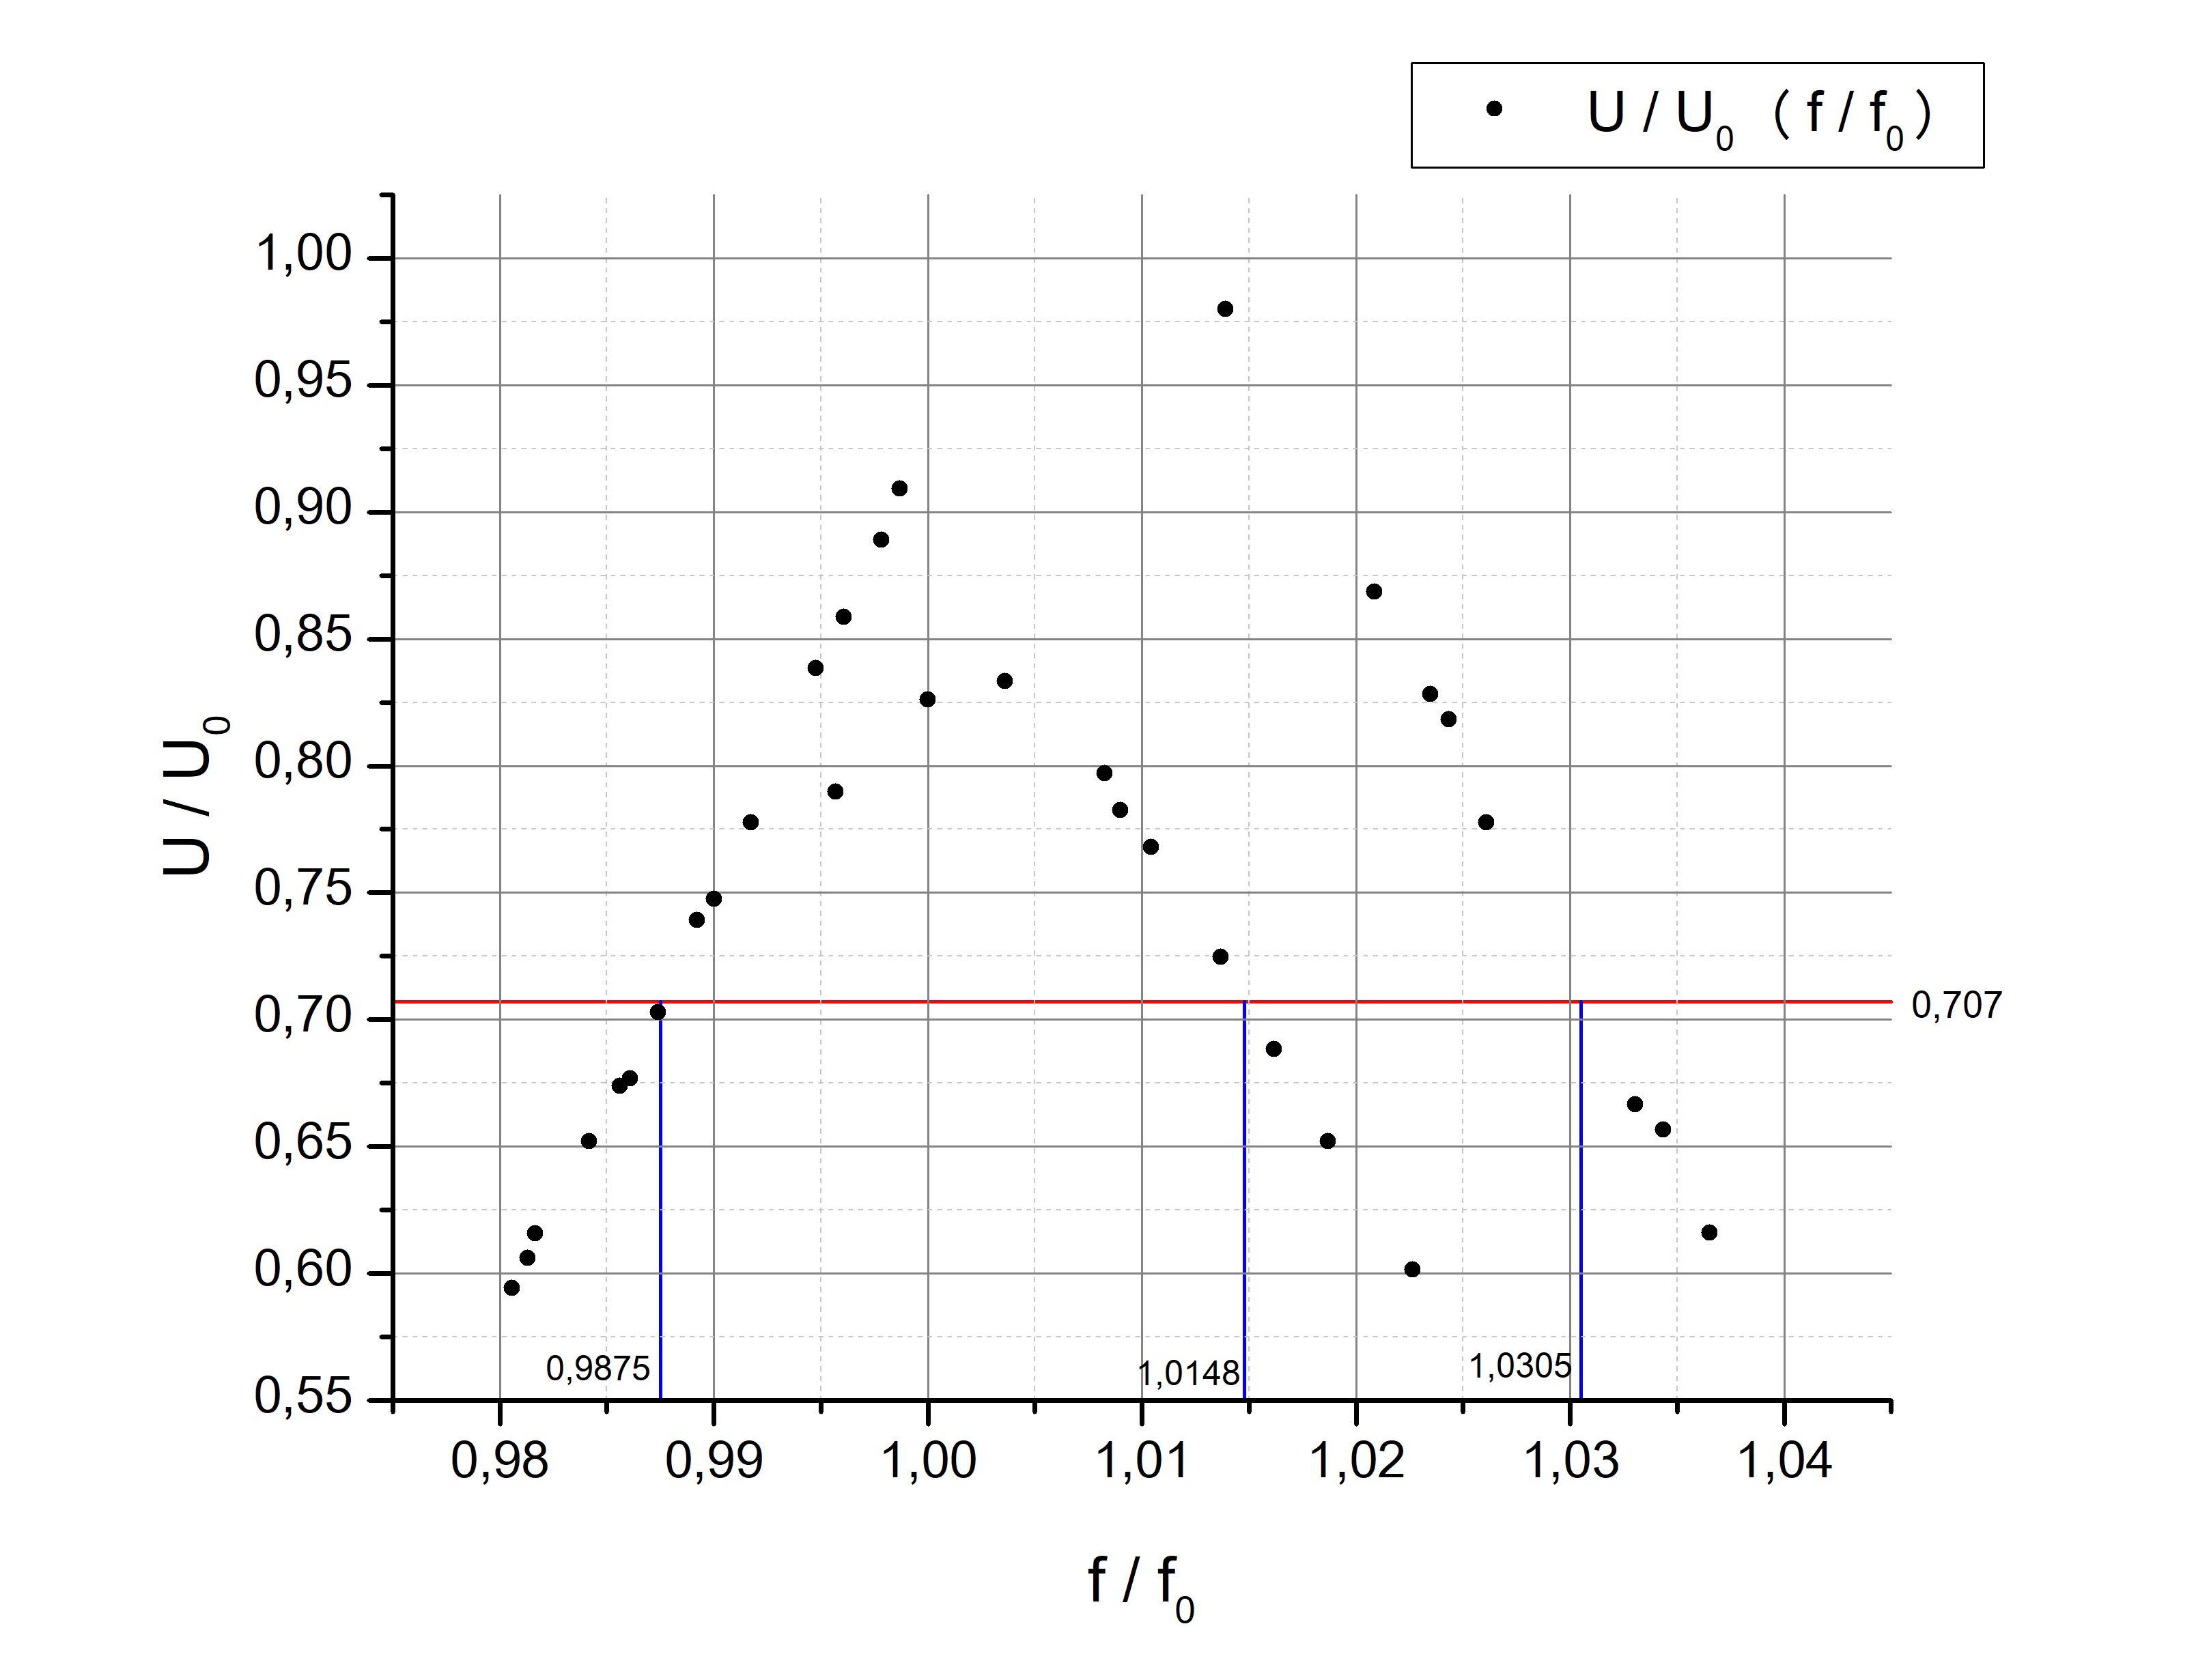
\includegraphics[scale=0.5]{АЧХ_2.png}}
	\caption{\centering График амплитудно-частотной характеристики в осях $\frac{U}{U_0} (\frac{f}{f_0})$}
	\label{fig:image2}
\end{figure}
Найдём добротность по ширине резонансной кривой для $C_2$ и $C_3$ соответственно:
\begin{equation}
    Q_2 = \frac{1}{df_2} = \frac{1}{1,01-0,99} = 36,63
\end{equation}
\begin{equation}
    Q_3 = \frac{1}{df_3} = \frac{1}{1,03-0,99} = 23,26
\end{equation}
\n\n
Составим фазово-частотную характеристику для конденсаторов $C_2$ и $C_3$. Будем определять разность фаз между сигналами $U(t)$, $\mathcal{E}(t)$ по следующей формуле:
\begin{equation}
    \psi_{\text{отн}} = \frac{x}{x_0} \psi
\end{equation}
Результаты занесём в таблицы
\begin{table}[H]
    \centering
    \caption{Результаты измерений ФЧХ для конденсатора $C_2$}
    \begin{tabular}{|l|l|l|l|l|l|}
    \hline
        $\psi$, рад & $f$, кГц & $x_0$, мкс & $x$, мкс & $f_{\text{отн}}$ & $\psi_{\text{отн}}$ \\ \hline
        -0,87 & 26,15 & 18,00 & 31,00 & 0,94 & -0,28 \\ \hline
        -1,05 & 26,33 & 18,00 & 30,00 & 0,95 & -0,33 \\ \hline
        -1,05 & 26,42 & 18,00 & 30,00 & 0,95 & -0,33 \\ \hline
        -0,87 & 27,10 & 18,00 & 31,00 & 0,97 & -0,28 \\ \hline
        -0,70 & 27,27 & 18,00 & 32,00 & 0,98 & -0,22 \\ \hline
        -0,35 & 27,56 & 18,00 & 34,00 & 0,99 & -0,11 \\ \hline
        -0,52 & 27,60 & 18,00 & 33,00 & 0,99 & -0,17 \\ \hline
        0,00 & 27,79 & 18,00 & 36,00 & 1,00 & 0,00 \\ \hline
        0,00 & 27,89 & 18,00 & 36,00 & 1,00 & 0,00 \\ \hline
        0,17 & 27,92 & 18,00 & 37,00 & 1,00 & 0,06 \\ \hline
        0,52 & 28,15 & 18,00 & 3,00 & 1,01 & 0,17 \\ \hline
        0,70 & 28,26 & 18,00 & 4,00 & 1,02 & 0,22 \\ \hline
        -0,17 & 28,40 & 18,00 & 35,00 & 1,02 & -0,06 \\ \hline
        1,05 & 28,78 & 18,00 & 6,00 & 1,04 & 0,33 \\ \hline
        1,22 & 29,04 & 18,00 & 7,00 & 1,04 & 0,39 \\ \hline
        1,05 & 29,39 & 18,00 & 6,00 & 1,06 & 0,33 \\ \hline
    \end{tabular}
\end{table}
\begin{table}[H]
    \centering
    \caption{Результаты измерений ФЧХ для конденсатора $C_3$}
    \begin{tabular}{|l|l|l|l|l|l|}
    \hline
        $\psi$, рад & $f$, кГц & $x_0$, мкс & $x$, мкс & $f_{\text{отн}}$ & $\psi_{\text{отн}}$ \\ \hline
        -1,14 & 22,04 & 22,00 & 36,00 & 0,96 & -0,36 \\ \hline
        -1,00 & 22,48 & 22,00 & 37,00 & 0,98 & -0,32 \\ \hline
        0,14 & 23,36 & 22,00 & 1,00 & 1,02 & 0,05 \\ \hline
        -0,86 & 22,72 & 22,00 & 38,00 & 0,99 & -0,27 \\ \hline
        -0,71 & 22,84 & 22,00 & 39,00 & 0,99 & -0,23 \\ \hline
        -1,00 & 22,13 & 22,00 & 37,00 & 0,96 & -0,32 \\ \hline
        -0,86 & 22,56 & 22,00 & 38,00 & 0,98 & -0,27 \\ \hline
        -0,86 & 22,62 & 22,00 & 38,00 & 0,98 & -0,27 \\ \hline
        -0,43 & 23,08 & 22,00 & 41,00 & 1,00 & -0,14 \\ \hline
        -0,29 & 23,12 & 22,00 & 42,00 & 1,01 & -0,09 \\ \hline
        0,00 & 23,22 & 22,00 & 0,00 & 1,01 & 0,00 \\ \hline
        0,29 & 23,47 & 22,00 & 2,00 & 1,02 & 0,09 \\ \hline
        0,57 & 23,53 & 22,00 & 4,00 & 1,02 & 0,18 \\ \hline
        0,86 & 23,78 & 22,00 & 6,00 & 1,03 & 0,27 \\ \hline
        0,71 & 23,64 & 22,00 & 5,00 & 1,03 & 0,23 \\ \hline
        1,00 & 24,20 & 22,00 & 7,00 & 1,05 & 0,32 \\ \hline
    \end{tabular}
\end{table}
По этим данным построим график фазово-частотной характеристики в осях $\psi_{\text{отн}}(f_{\text{отн}})$
\begin{figure}[H]
	\center{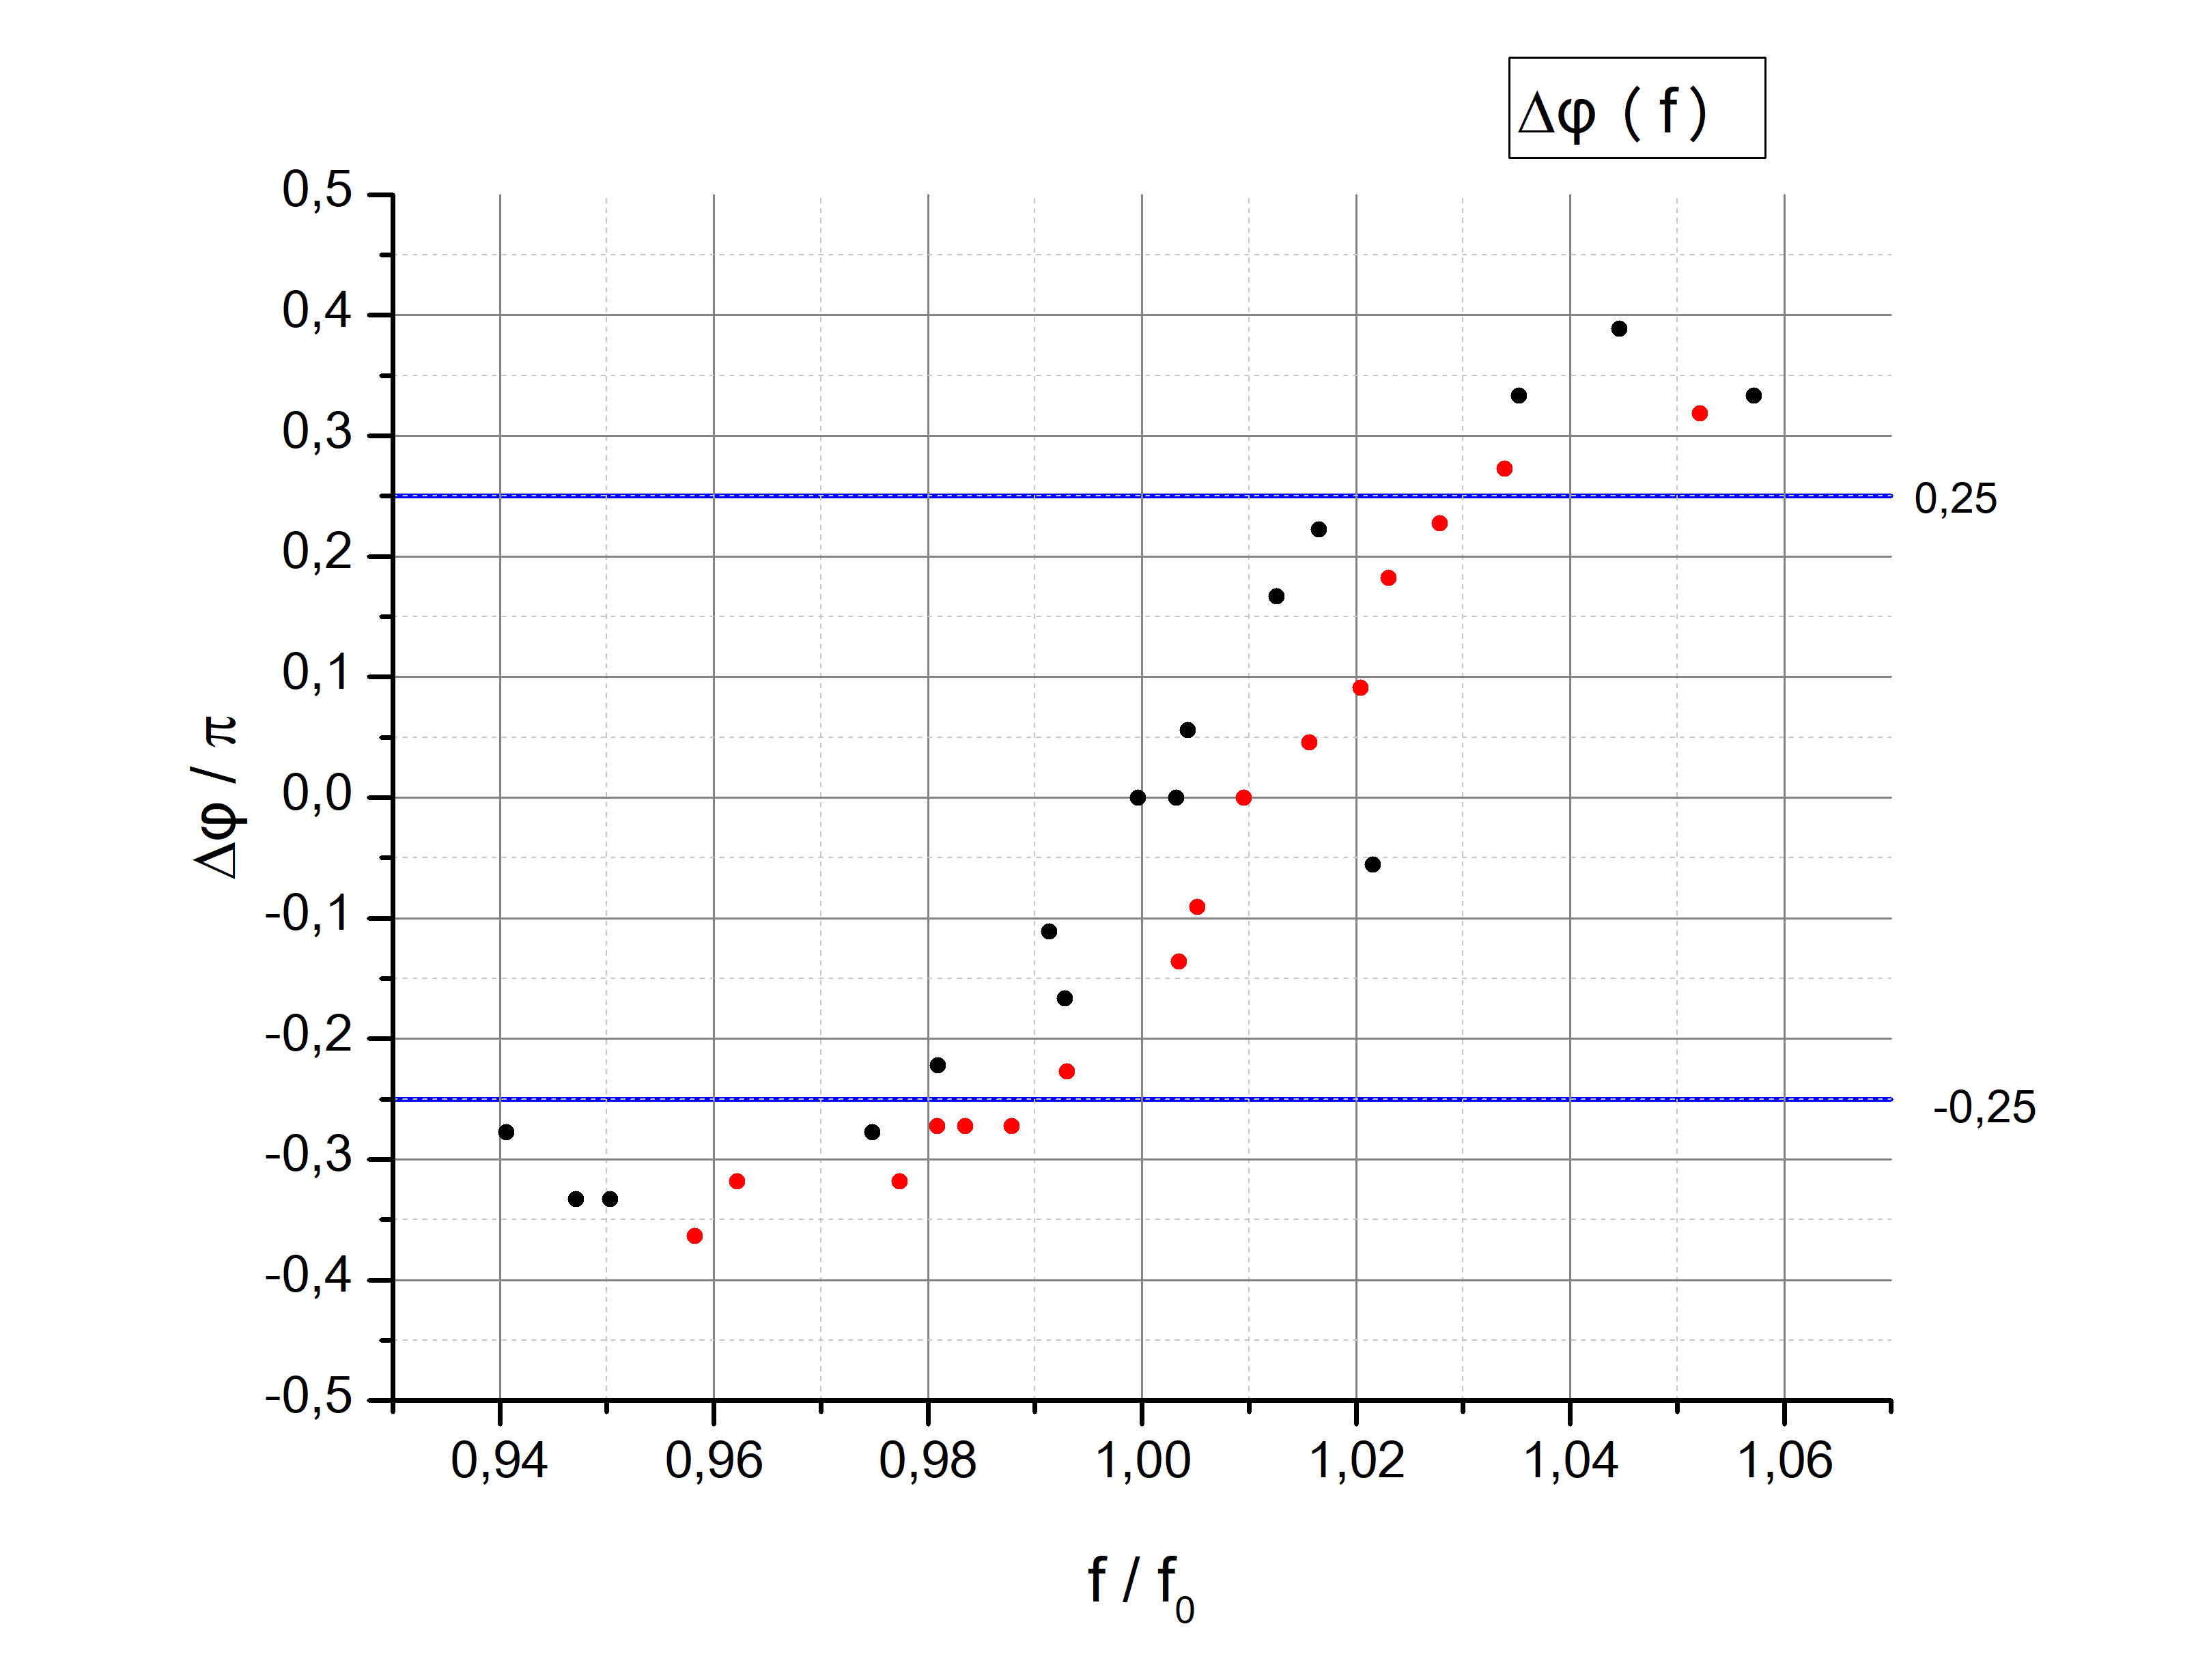
\includegraphics[scale=0.5]{ФЧХ.png}}
	\caption{\centering График фазово-частотной характеристики в осях $\psi_{\text{отн}}(f_{\text{отн}})$}
	\label{fig:image2}
\end{figure}
Определим добротности контуров по расстоянию между точками оси x:
\begin{equation}
    Q_2=\frac{1}{dx}=\frac{1}{1,02-0,98}=25
\end{equation}
\begin{equation}
    Q_3=\frac{1}{dx}=\frac{1}{1,03-0,99}=25
\end{equation}
Далее построим график зависимости $R_L(f_{0n})$ и нанесём на график прямую $\langle R_L \rangle$.
\begin{figure}[H]
	\center{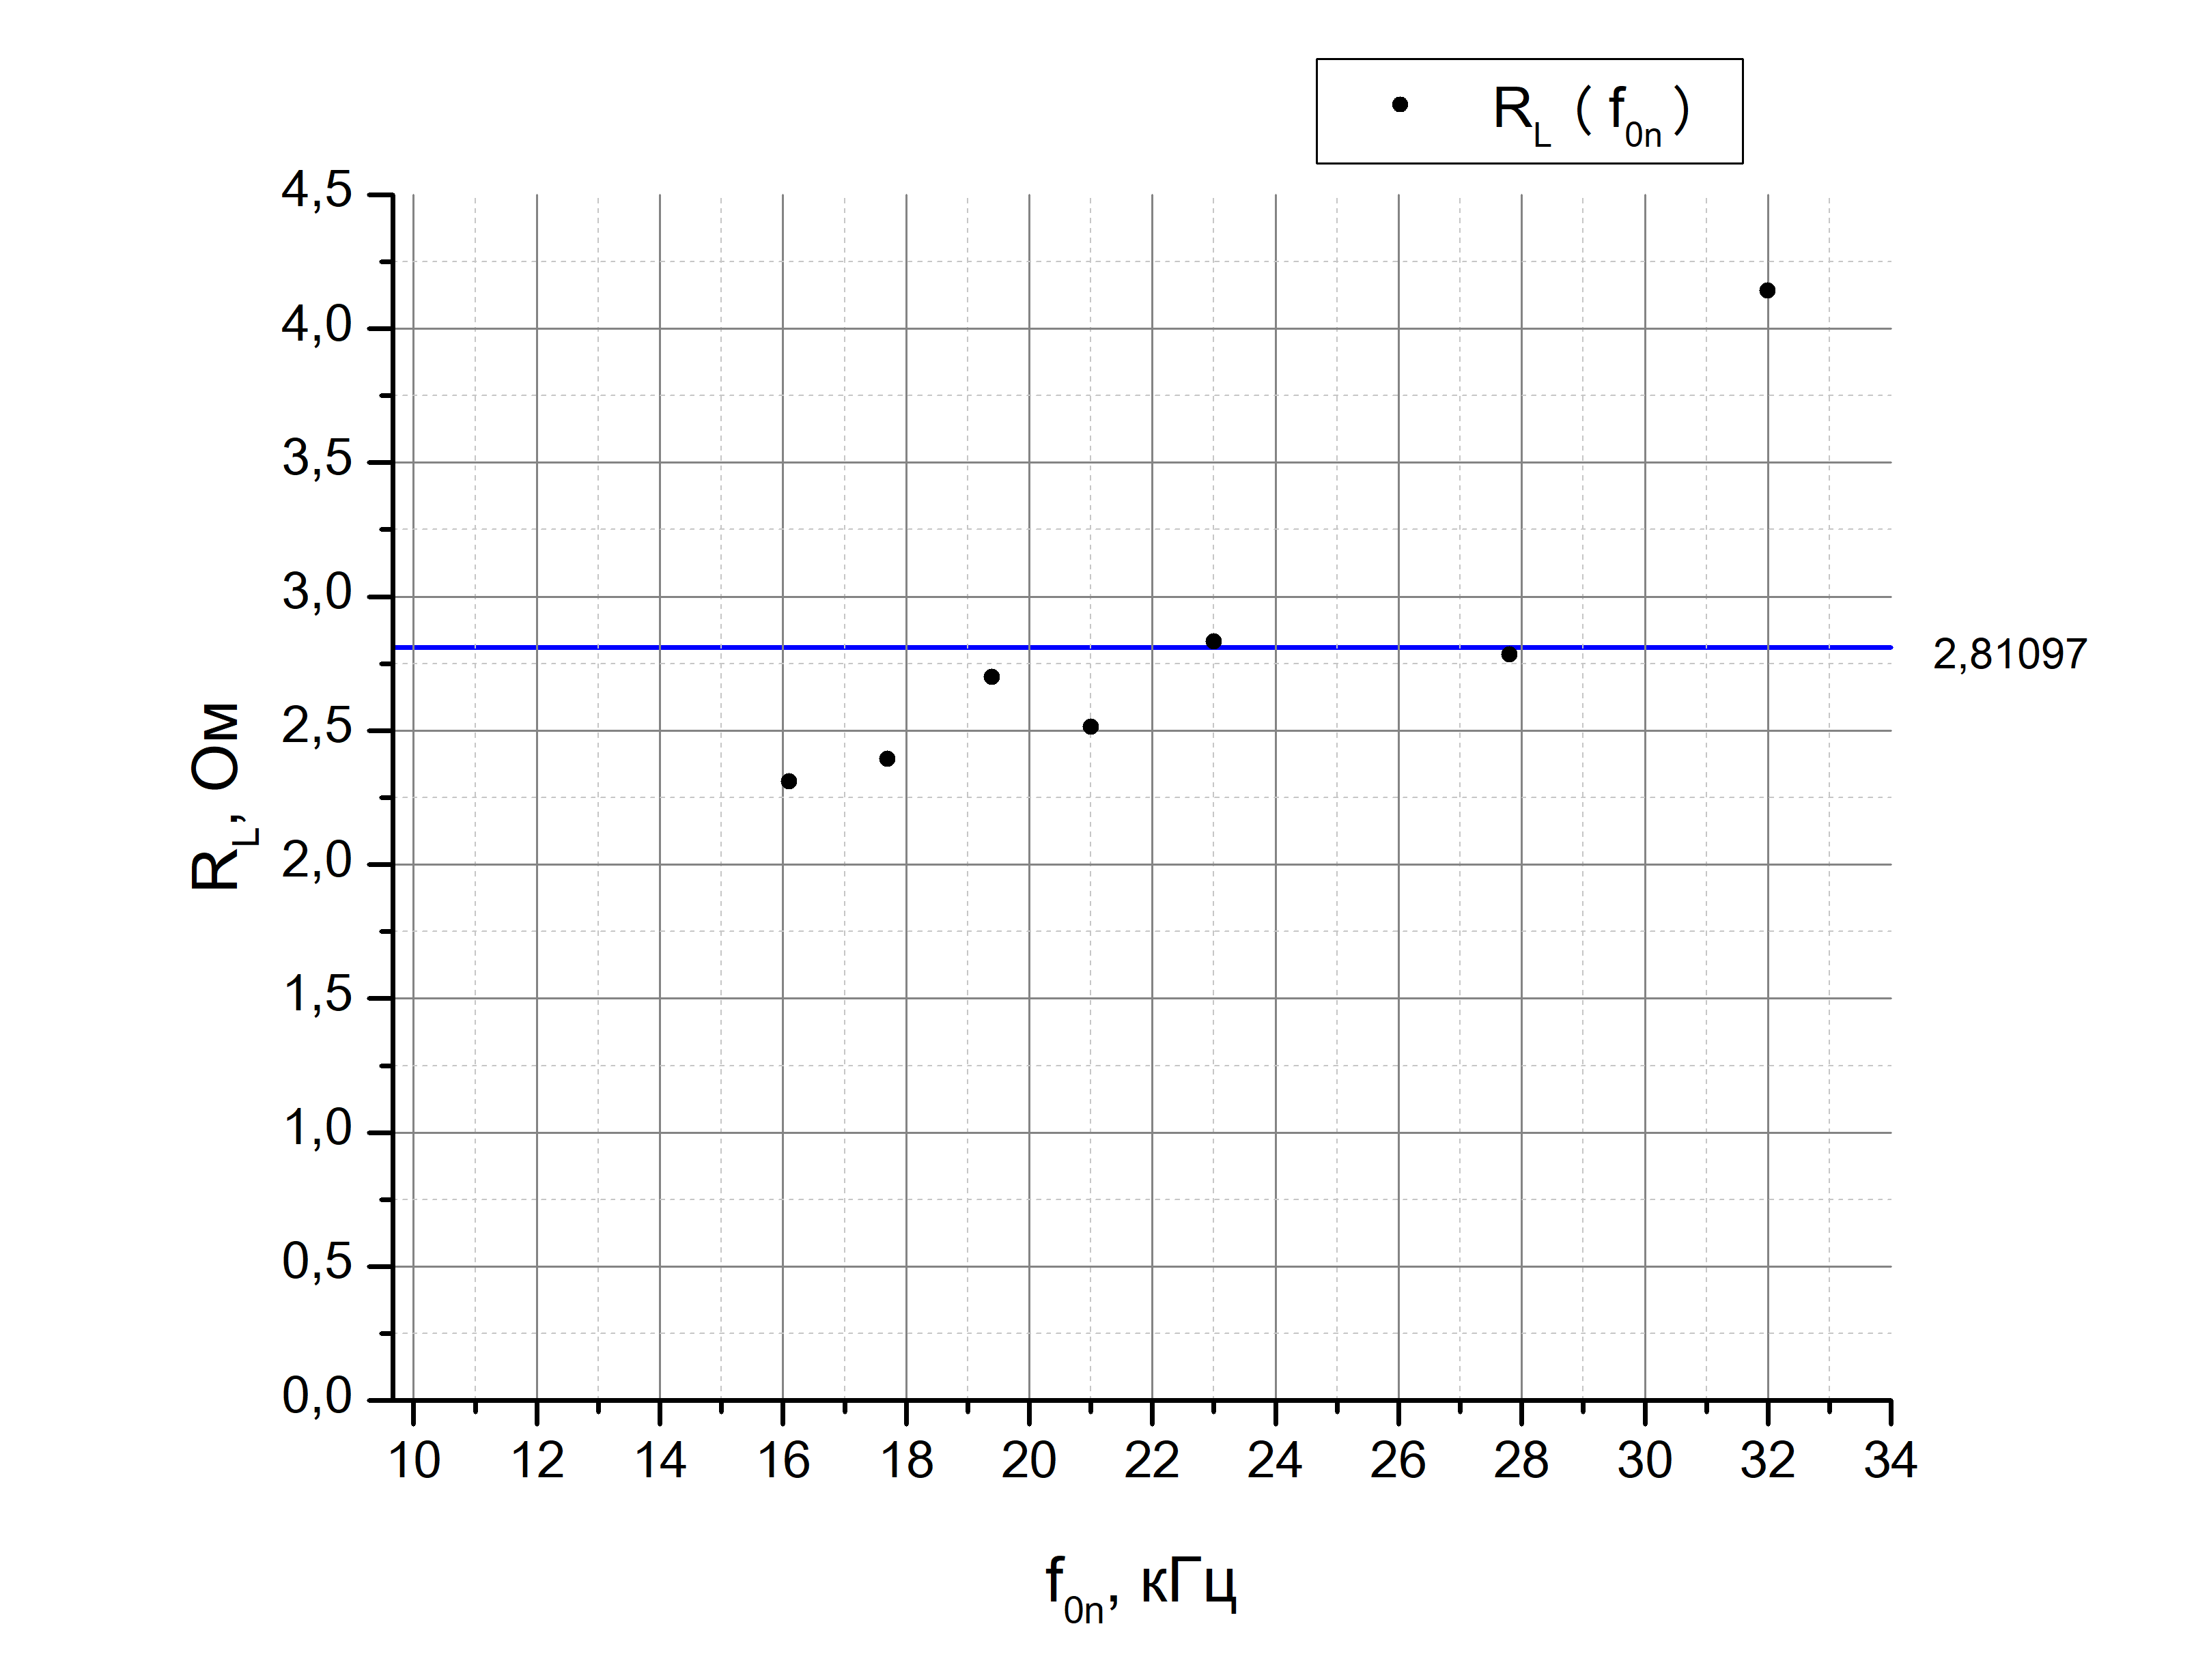
\includegraphics[scale=0.4]{R_L.png}}
	\caption{\centering график зависимости $R_L(f_{0n})$ с прямой $\langle R_L \rangle$}
	\label{fig:image2}
\end{figure}
\n\n
Берём $Q_7 = 16,47$ - контур с наименьшей добротностью. Посчитаем ток по формуле:
\begin{equation}
    I = \frac{\mathcal{E}}{R_1} = 0,3 \ \text{мА}
\end{equation}
Его вектор равен $\Vec{I}=\Vec{I_L} + \Vec{I_C}$ и расположен на оси абсцисс. Построим векторную диаграмму.
	\begin{figure}[H]
	\center{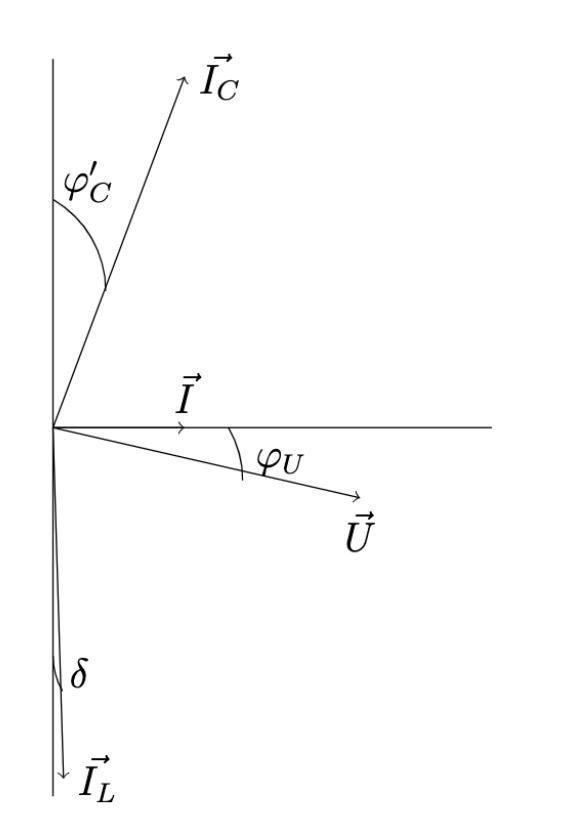
\includegraphics[scale=1.3]{DIAGRAM.jpg}}
	\caption{\centering векторная диаграмма}
	\label{fig:image2}
\end{figure}
	\n
	Далее:
	\[\varphi^{'}_C = \frac{R + R_{l}}{\rho} \approx 0.06\]
	\[\varphi_U = - \frac{R + R_{l}}{\rho} \approx - 0.06\]
	\subsection*{Вывод}
	В данной работе мы изучили резонанс токов в параллельном контуре. С помощью непосредственных измерений, графиков АЧХ и ФЧХ мы определили добротность контуров и получили хорошо совпадающие результаты. 
\n\n
В конце работы мы построили векторную диаграмму как наглядное представления "<резонанса токов">. 

\end{document}